\documentclass{article}

\usepackage{amsmath,amsthm,amssymb}
\usepackage{fullpage}
\usepackage{enumerate}
\usepackage{hyperref}
\usepackage{graphicx}

\DeclareMathOperator{\lcm}{lcm}


\begin{document}

\setlength{\tabcolsep}{0.015\textwidth}
\begin{center} \begin{tabular}{cccc}
	
\includegraphics[width=0.16\textwidth]{SAMF_logo.jpg} &
	
\includegraphics[width=0.35\textwidth]{SAICA_logo.jpg} &
	
\includegraphics[width=0.18\textwidth]{Liberty_logo.jpg} &
	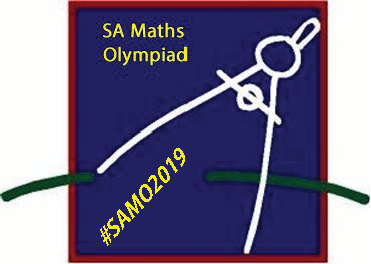
\includegraphics[width=0.18\textwidth]{SAMO2019.png}
\end{tabular} \end{center}


\vspace{30pt}

\begin{center}
\textbf{\Large Intermediate January Monthly Problem Set}
\\ \vspace{1em}
\textbf{\large Due: 25 January 2019}
\end{center}

\vspace{12pt}

\begin{enumerate}[1.]

\item % IPMO 2006 Junior Team Q4
\[ \sqrt[3]{\frac{2+1}{2}\cdot\frac{3+1}{3}\cdot\frac{4+1}{4}\dotsm\frac{a+1}{a}} = 4. \]
Find the value of $a$.


\item % SW-2009-5
In a triangle $ABC$, let $D$ and $E$ be the midpoints of $AB$ and $AC$, respectively, and let $F$ be the foot of the altitude through $A$. Show that the line $DE$, the angle bisector of $\angle ACB$ and the circumcircle of $ACF$ pass through a common point.


\item % IPMO 2005 Junior Team Q6
Determine the number of triplets $(k,l,m)$ of positive integers such that
\begin{align*}
  k+l+m &= 97 \quad \mathrm{and} \\
  \frac{4k}{5} +\frac{5l}{6} +\frac{6m}{7} &= 82.
\end{align*}


\item % DB-2012-1
A positive integer is called \emph{special} if its digits can be arranged to form an integer divisible by $4$. How many of the integers from $1$ to $2018$ are special?


\item % JM-2009-3 part (a)
Prove that if $p > 10$ is a prime number that divides $a^4+a^3+a^2+a+1$ for some integer $a$, then $p$'s decimal expansion ends in a $1$.


\item % SW-2007-3
Steve determines the geometric mean of two positive integers in the following way:
\begin{enumerate}
	\item He writes them down in their decimal representation, one below the other, and prepends zeros to the smaller number (if applicable) such that their lengths are equal.
	\item He determines the geometric mean of each pair of digits below each other. If the result is not an integer, only the integer part is used.
	\item The digits determined by this procedure form the result.
\end{enumerate}
Determine all pairs $(a,b)$ of positive integers for which Steve's procedure yields the correct result. (For example, one such pair is $(12; 48)$.)


\item % SW-2008-1
The set $S$ of nonnegative integers has the property that every nonnegative integer $n$ can be uniquely written as $n = a+2b$ where $a,b \in S$ are not necessarily distinct. How many elements of $S$ are less than $2018$?


\item % SH-2006-1
$P$, $Q$ and $R$ are any points on $BC$, $CA$ and $AB$ respectively of a triangle $ABC$. Let the centres of the circumcircles $AQR$, $BRP$ and $CPQ$ be $X$, $Y$ and $Z$. Prove that triangles $XYZ$ and $ABC$ are similar.


\end{enumerate}


\vfill
\textbf{\Large Email submission guidelines}
\begin{itemize}
	\item Email your solutions to \href{mailto:samf.training.assignments@gmail.com}{\texttt{samf.training.assignments@gmail.com}}.
	\item In the subject of your email, include your name and the level of the assignment (Beginner, Intermediate or Senior).
	\item Submit each question in a single separate PDF file (with multiple pages if necessary), with your name and the question number written on each page.
	\item If you take photographs of your work, use a document scanner such as CamScanner to convert to PDF.
	\item If you have multiple PDF files for a question, combine them using software such as PDFsam.
\end{itemize}

\end{document}
